% IEEE workshop paper — controlled policy-selector study for malleable GPU scheduling.
% Build: cd Research/paper && latexmk -pdf ieee.tex
% 2026-09-13: aligned with the frozen core-2x2-v1 protocol.  Partial validation results
% are labelled exploratory; no test-split or interaction claim is made.
\documentclass[conference]{IEEEtran}
\usepackage{graphicx}
\usepackage{booktabs}
\usepackage{amsmath}
\usepackage{url}
\usepackage{xcolor}
\usepackage{tikz}
\usetikzlibrary{arrows.meta,positioning,shapes.geometric}

\newcommand{\todo}[1]{\textcolor{red}{\textbf{[TODO: #1]}}}
% * = 95% CI excludes 0, paired by seed, n=32
\newcommand{\sig}{$^{*}$}

\begin{document}

\title{Do Multi-LLM Referees Improve Malleable GPU Scheduling?\\
A Controlled Market/Reasoning Factorial Study}

\author{\IEEEauthorblockN{Lay Kim Seng}
\IEEEauthorblockA{Cyberscience Center, Tohoku University\\
lay.kim.seng.q4@dc.tohoku.ac.jp}
\and
\IEEEauthorblockN{\todo{co-authors / advisor}}
\IEEEauthorblockA{~}}

\maketitle

\begin{abstract}
We study whether two commonly proposed additions to GPU scheduling --- market-based allocation
and multi-LLM role separation --- improve decisions once jobs are allowed to resize.  The frozen
experiment is a $2\times2$ factorial design: a Single Referee or Demand--Supply--Referee structure
selects from either four non-market rules or four uniform-price auction valuations, together with
one of four sizing actions.  Every cell uses the same Qwen2.5-14B model, parser, state, decoding
budget, paired seeds, synthetic deadlines, and $80$-GPU MIT Supercloud trace windows.  At the
experiment cutoff, 477 of 1,056 planned runs had completed, all on validation windows.  The two
complete Single-Referee cells differ by only $-0.40$ percentage points in deadline violations in
favour of the market family (95\% CI $[-1.25,0.45]$, exact $p=0.438$, 12 paired windows).  The
Multi-Market cell is absent and Multi-Non-market lacks two of three seeds, so the preregistered
multi-agent and interaction hypotheses are not estimable.  Strong fixed policies are already
competitive: FAIR+ADAPT reaches $10.49\%$ and Auction-Deadline+ADAPT $9.87\%$ validation
violations, versus $11.59\%$ and $11.19\%$ for the corresponding single referees.  A separate
counterfactual library of 1,092 deterministic rollouts yields 44 clean training states and 24
held-out validation states for Qwen3-8B LoRA.  Its oracle improves the fixed non-market baseline
by $2.03$ points on validation but the market baseline by only $0.07$ points; the median gain is
zero in both families.  Fine-tuning does not realise this ceiling: held-out mean regret is $8.78$
points versus $8.70$ zero-shot and $1.05$ for the fixed floor, with 11/24 malformed outputs from
both model arms.  Thus the current evidence supports safe adaptive sizing, but not a claim that
markets, multi-agent reasoning, or this small LoRA intervention improves scheduling.
\end{abstract}

\begin{IEEEkeywords}
GPU scheduling, large language models, resource allocation, multi-agent debate, cluster traces
\end{IEEEkeywords}

\section{Introduction}

AI training and inference are the dominant consumers of GPU clusters, and they are
\emph{elastic}: a training job can run on more or fewer devices, trading device-hours against
completion time. A scheduler on such a workload therefore makes two decisions per job, not one
--- \emph{which} job to start, and \emph{how large} to make it.

Almost every published evaluation erases the second decision. A trace records that a job used
$g$ devices for $t$ seconds; it does not record what that job would have done on $2g$ or on
$g/2$, because the counterfactual was never observed. The standard response is to replay the
trace \emph{rigidly}, pinning each job to its historical size. This is usually presented as a
conservative simplification. We show it is a suppression, and that it silently invalidates the
efficiency claims most commonly made on top of it.

The argument is short. If no job can be resized, the device-seconds a workload consumes are
fixed: every scheduler must run the same jobs for the same durations, so it can only move work
earlier or later. Utilisation is then close to a conserved quantity, and a comparison of
schedulers on it is close to a comparison of nothing. Restoring elasticity does not merely add
a tuning knob; it makes utilisation controllable, and --- as we show --- makes maximising it
actively harmful.

Our contributions, all on the MIT Supercloud GPU trace replayed through a malleability-aware
batch simulator~\cite{elastisim}, are:
\begin{enumerate}
\item \textbf{A controlled policy-selector test} (\S\ref{sec:factorial-method}).  We freeze a
$2\times2$ design that separates policy family (market/non-market) from reasoning structure
(Single/Multi), holds the action space and model configuration fixed, and pairs windows and seeds.
\item \textbf{A reportable negative stopping result} (\S\ref{sec:factorial-results}).  The only
complete factorial contrast, market versus non-market under a Single Referee, is small and
uncertain.  The run does not contain enough evidence to estimate a Multi effect or interaction.
\item \textbf{A deterministic floor and oracle ceiling} (\S\ref{sec:oracle}).  Strong fixed
ADAPT policies match the zero-shot referee closely.  Counterfactual enumeration finds modest
non-market headroom but almost none for the market family, localising what a learned selector
could still improve.
\item \textbf{A diagnostic explanation for the result} (\S\ref{sec:sizing}).  Prior controlled
replays show that sizing dominates ordering and that occupancy-maximising GREEDY sizing is harmful;
the useful decision is safe sizing under uncertainty, rather than unconstrained LLM allocation.
\end{enumerate}

We additionally retain, unchanged, a result that does not depend on any trace
(\S\ref{sec:text}): on an authored suite of exceptions expressible only in operator text ---
which no public GPU trace supplies --- a debate between LLM reviewers corrects a single model's
rulings at an identical call budget. That is where a reasoning layer earned its cost in our
setting; it is not the numeric rationing decision, and \S\ref{sec:antimetric} explains why the
numeric decision has been measured against the wrong target.

\section{Related Work}
\label{sec:related}

\textbf{LLM-driven scheduling.} LLMsched~\cite{llmsched} repairs a single LLM's proposal with
an ILP and reports large gains over Kubernetes. We inherit the reason-then-guarantee spine but
invert its default: on numeric rationing the deterministic layer should be the proposer, not
just the repairer, and the LLM should be gated behind a contextual trigger.
\todo{2--3 more LLM-scheduling refs}

\textbf{Learning-based schedulers.} DRL schedulers (DeepRM~\cite{deeprm},
Decima~\cite{decima}) learn allocation policies but are black-box and brittle under
distribution shift. On our interface a tabular Q-learner's episode-return variance dominates
the action effect at realisable sample counts.

\textbf{Multi-agent LLM structures.} Multiagent debate~\cite{du2024debate} and
self-consistency~\cite{wang2023selfconsistency} are usually evaluated on QA benchmarks, and
LLM-as-judge protocols~\cite{zheng2023judge} inherit that setting; budget-matched controls are
rare, so a reported gain is rarely separable from the extra calls that buy it. Our
text-exception result is budget-matched by construction and includes a blind confirmatory
batch.

\textbf{Malleability and mechanism design.} Runtime elasticity is rarely deployed in
production~\cite{tarraf2024}; our partial-allocation model rests on it and we state that
dependence. Uniform-price auctions are the classical route to truthful revelation, and
automated negotiation for resource allocation is a classical subject~\cite{boan2011}, with
prediction-guided \emph{selective} negotiation explored in one-shot fair
division~\cite{croitoru2025}; our contribution is measurement in a closed loop containing
declarative LLM agents.

\section{Controlled Policy-Selector Architecture}
\label{sec:arch}

\begin{figure}[t]
\centering
\resizebox{\columnwidth}{!}{%
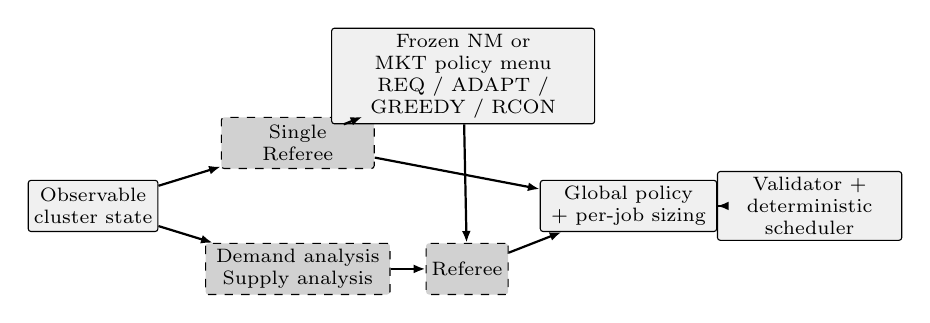
\begin{tikzpicture}[
  font=\scriptsize,
  box/.style={draw, rounded corners=1pt, align=center, minimum height=6.5mm, inner sep=2pt},
  code/.style={box, fill=black!6},
  llm/.style={box, fill=black!18, dashed},
  gate/.style={diamond, draw, aspect=2, align=center, inner sep=1pt},
  arr/.style={-{Latex[length=1.5mm]}, thick},
  lab/.style={font=\tiny, fill=white, inner sep=1pt},
]
\node[code] (state) at (0,0) {Observable\\cluster state};
\node[llm, text width=1.8cm] (single) at (2.6,0.8) {Single\\Referee};
\node[llm, text width=2.2cm] (roles) at (2.6,-0.8) {Demand analysis\\Supply analysis};
\node[llm] (ref) at (4.75,-0.8) {Referee};
\node[code, text width=2.1cm] (action) at (6.8,0) {Global policy\\+ per-job sizing};
\node[code, text width=2.2cm] (apply) at (9.1,0) {Validator +\\deterministic scheduler};
\node[code, text width=3.2cm] (menu) at (4.7,1.65) {Frozen NM or MKT policy menu\\REQ / ADAPT / GREEDY / RCON};
\draw[arr] (state) -- (single);
\draw[arr] (state) -- (roles);
\draw[arr] (roles) -- (ref);
\draw[arr] (single) -- (action);
\draw[arr] (ref) -- (action);
\draw[arr] (menu) -- (single);
\draw[arr] (menu) -- (ref);
\draw[arr] (action) -- (apply);
\end{tikzpicture}
}
\caption{The controlled $2\times2$ pipeline.  Single and Multi arms receive the same observable
state and frozen action menu.  Demand and Supply agents produce analysis only; the Referee is the
sole decision-maker.  All outputs pass through the same deterministic feasibility layer.}
\label{fig:pipeline}
\end{figure}

Fig.~\ref{fig:pipeline} shows the two reasoning structures.  At each 1,800-second selection
point the model sees available capacity and scheduler-visible attributes of pending and running
jobs: arrival and waiting time, requested walltime and GPU count, priority, deadline pressure,
legal malleable bounds, and scaling indicators.  It never sees true runtime or future arrivals.

\textbf{Single Referee.} One model returns strict JSON containing one global ordering policy, a
default sizing rule, and optional job-specific sizing overrides.  The parser expands this into
exactly one action for every affected job.

\textbf{Demand--Supply--Referee.} Demand identifies urgent, deadline-pressured, scalable, and
shrink-tolerant jobs. Supply describes scarcity, queue pressure, resize cost, and fairness.  These
agents cannot allocate GPUs; their analyses and the original state are passed to a Referee whose
output schema is identical to the Single arm.

\textbf{Frozen action and safety layers.} The non-market menu is FCFS, least-laxity, ageing
fair-share, and priority-tier FCFS.  The market menu holds the auction mechanism fixed and varies
the observable valuation: wait, deadline, fair-share, or priority.  Both expose REQ, ADAPT,
GREEDY, and resize-conservative (RCON) sizing.  A shared validator rejects malformed actions,
enforces the $80$-GPU capacity and each job's legal bounds, and invokes a counted deterministic
fallback.  Hence the factorial comparison changes only policy family and reasoning structure.

\section{Evaluation}
\label{sec:eval}

\textbf{Setup.} We replay the MIT Supercloud GPU trace (a $235$-day Slurm accounting log)
through ElastiSim~\cite{elastisim}, a batch-system simulator for malleable workloads. One
simulated node is one GPU, so a job that used $g$ GPUs becomes a $g$-node job; its work is set
so that it reproduces its recorded runtime exactly. The scheduler sees each job's arrival, size
and \emph{requested} walltime, never its true runtime --- the same information a production
batch system has. Capacity is a fixed $80$-GPU pool, so a window's offered load is a property
we \emph{measure} rather than a consequence of sizing the cluster to fit it.

\textbf{Window selection is pre-registered.} Every $24$\,h window of the trace is described by
workload statistics alone --- job count, GPU-hours, offered load, high-priority fraction,
median and p90 runtime, size distribution --- with no scheduler executed. Of $5{,}613$ hourly
starts, $4{,}312$ carry at least $100$ jobs. These are stratified into four offered-load bands
($0.7$--$1.0$, $1.0$--$1.5$, $1.5$--$2.5$, ${>}2.5\times$) crossed with three high-priority
bands (${<}2\%$, $2$--$10\%$, ${>}10\%$), and one window is drawn per cell under a fixed seed,
subject to a non-overlap constraint. The resulting $12$ windows span days $41$--$222$, offered
loads $0.75$--$4.97\times$ and priority fractions $0.7$--$58\%$. Each is preceded by $12$\,h of
warm-up arrivals, which the arm under test also schedules but which are excluded from scoring,
so no run begins on an empty cluster. Selection never sees a scheduler result.

\textbf{Elasticity model.} A job may be \emph{moldable}: its size is chosen once, at launch, and
fixed thereafter. Speed-up follows Amdahl's law anchored on the observed point --- a job seen at
$g$ GPUs reproduces its recorded runtime exactly at $g$, so the rigid replay is this same model
evaluated at the size the job really ran, and the parallel fraction $s$ is swept rather than
assumed ($s{=}1$ is rigid at every size, $s{=}0$ is linear speed-up). Results below use
$s{=}0.7$, a deliberately conservative value: scaling is sublinear, so growing a job costs more
device-time than it saves. We report SLA-$k$ (turnaround exceeding $k\times$ true runtime) at
$k \in \{2,5,10\}$, mean waiting time, device-hours actually spent, walltime kills, and
occupancy over the measured window.

\subsection{Frozen factorial protocol}
\label{sec:factorial-method}

The core experiment uses 48 non-overlapping 24-hour windows, each with 12 hours of warm-up,
selected from workload characteristics before scheduling outcomes are inspected.  They are frozen
as 24 train, 12 validation, and 12 test windows.  Every scored window contains at least 100 jobs.
Jobs are malleable at ten resize points with bounds
$1\leq g_i(t)\leq\min(80,4g_i^{\mathrm{trace}})$, $s=0.7$, and no modeled resize overhead.
Synthetic deadlines are generated once as
$D_i=a_i+W_i^{\mathrm{req}}$; a missing walltime receives the fixed 86,400-second estimate.
Deadline violation rate is the primary outcome.

The four inferential cells are Single-NM, Single-MKT, Multi-NM, and Multi-MKT.  Qwen2.5-14B is
held fixed at temperature 0.1 and a 400-token output limit.  Thirty-two deterministic controls
exhaustively cross the four policies and four sizing actions in each family.  Validation selects
the best fixed policy per family; test is reserved for one final report.  The inferential unit is
the window.  The preregistered analysis contains exactly three two-sided paired contrasts on test:
market main effect, Multi main effect, and their difference-in-differences interaction.  It uses
paired-$t$ 95\% confidence intervals, exact sign-flip tests, and Holm correction over these
contrasts.

Two amendments to the frozen protocol are recorded with it rather than absorbed silently.  The
first corrects the feasibility assertion, which excluded completed jobs but not killed ones from
simultaneous-ownership accounting and so aborted otherwise valid runs; it changes no ordering,
sizing, bid, deadline, window, or reported metric.  The second reduces the inference seed set from
three seeds to one.  The multi-agent cell costs $1{,}703$\,s per window run against $251$\,s for
the single referee and $8$\,s for a deterministic control, so the three-seed design needed a
further $64$ hours of inference.  With one response per window, within-window response noise is no
longer separable from between-window variance, and at temperature $0.1$ a single response is a draw
rather than a deterministic answer; the paired tests are therefore more conservative, not less.
The protocol plans 864 runs: 768 fixed-policy and 96 LLM-controlled runs over validation and test.

Every result row stores hashes of the processed trace, the generated world, the implementation, the
manifest, and the Git revision, and a fail-closed gate re-checks all of them, together with the
split, window non-overlap, per-job deadlines, malleable bounds, and speedup-curve anchoring, before
any run executes.  Superseded hashes are retained explicitly, so rows produced before an amendment
remain verifiable instead of being restamped.  Runtime assertions enforce cluster capacity,
malleable bounds, nonnegative remaining work, and single completion at every scheduler invocation.

\subsection{The rigid replay cannot answer an efficiency question}
\label{sec:rigid}

With every job pinned to its historical size, the device-seconds consumed are fixed by the
window, not chosen by the scheduler. Empirically this leaves almost nothing to compete over.
Across five schedulers (strict FCFS, first-fit, EASY backfilling, requested-walltime ordering,
and a declared/undeclared split) occupancy differs by at most $1.3$ points within a window and
is identical to three decimal places in several. The idle capacity any ordering rule could
still recover --- devices free while a job that fitted was waiting --- averages $0.2\%$, with a
worst case of $1.3\%$.

Service quality is equally flat. Over $11$ windows no arm separates from the EASY baseline
after Holm correction across three SLA thresholds; the largest raw effect, $-4.2$ points of
SLA-2, carries $p_{\text{Holm}}=0.41$. Two properties of the trace explain the flatness and are
worth recording, because both are usually assumed away. First, EASY backfilling is inert here:
across $1{,}351$ blocked scheduling points it backfilled $48$ times ($3.6\%$), because
requested walltimes exceed true runtimes by $100$--$600\times$, so no job can be shown to fit
before the head job's reservation. EASY and strict FCFS are byte-identical on most windows.
Second, requested walltime carries no runtime signal: among $487$ jobs in one window there are
$9$ distinct requested values, and the rank correlation with true runtime is $+0.16$, $-0.11$,
$-0.73$ and $-0.01$ across four windows --- the only significant value is negative. Any
``shortest-job-first'' arm on this trace is therefore ordering on noise.

\subsection{Made elastic, sizing dominates ordering}
\label{sec:sizing}

We now allow every job to be moldable and hold the ordering rule fixed at first-fit, varying
only how each job is sized: \textsc{as-requested} honours the size its owner asked for and
waits until that many devices are free; \textsc{greedy} takes the largest legal size that fits;
\textsc{adaptive} shares free capacity across the waiting queue. Table~\ref{tab:sizing} reports
means over the $12$ pre-registered windows.

\begin{table}[t]
\centering
\caption{Sizing rule, $12$ pre-registered windows, $s=0.7$, first-fit ordering held fixed.
Mean $\pm$ 95\% CI.}
\label{tab:sizing}
\small
\resizebox{\columnwidth}{!}{%
\begin{tabular}{lrrrr}
\toprule
sizing & device-h & occupancy & SLA-10 (\%) & mean wait (s) \\
\midrule
\textsc{as-requested} & $3653$ & $0.890$ & $22.3$ & $38{,}072$ \\
\textsc{adaptive}     & $3339$ & $0.964$ & $32.5$ & $39{,}756$ \\
\textsc{greedy}       & $9581$ & $0.988$ & $76.2$ & $270{,}522$ \\
\bottomrule
\end{tabular}
}
\end{table}

The spread is an order of magnitude, on an axis that does not exist in the rigid replay. Paired
against \textsc{as-requested}, \textsc{greedy} costs $+5{,}929 \pm 1{,}707$ device-hours
($p{=}3\times10^{-5}$), $+232{,}451 \pm 60{,}823$\,s of mean waiting ($p{=}10^{-5}$) and
$+53.9 \pm 12.3$ points of SLA-10 ($p{<}10^{-5}$). No ordering rule we measured in
\S\ref{sec:rigid} moves any metric by a comparable amount.

\subsection{Utilisation is an anti-metric}
\label{sec:antimetric}

The three sizing rules order identically on occupancy and inversely on service.
\textsc{greedy} attains the \emph{highest} occupancy of any arm we measure --- $0.988$, against
$0.890$ for \textsc{as-requested} ($+0.1 \pm 0.1$, $p{=}0.009$) --- while being the worst on
every service axis simultaneously. In $12$ of $12$ windows the highest-occupancy arm is the
worst-service arm, and in $10$ of $12$ the highest-occupancy arm is not the best-service arm.

The mechanism is not subtle, which is what makes the metric dangerous. Under sublinear scaling,
a job given $4\times$ the devices at $s{=}0.7$ finishes about $1.6\times$ sooner while
consuming $4\times$ the capacity. \textsc{greedy} therefore converts the cluster into
\emph{busy-ness} without converting it into completed work, and the queue behind it grows.
Occupancy records the busy-ness and is blind to the waste: on one low-load window it reads
$1.000$ for all three sizing rules while their mean waiting times span $21{,}429$\,s to
$244{,}781$\,s.

This is the practical consequence of \S\ref{sec:rigid}. A rigid replay reports occupancy
differences of a fraction of a point and no scheduler can game them; the metric looks harmless
because it is inert. Made elastic, the same metric becomes controllable --- and the controller
that maximises it is the one to avoid. We therefore recommend reporting device-hours spent per
unit of completed work, together with waiting time, and retiring occupancy as a headline number
for elastic workloads.

\subsection{Sizing under uncertainty is open, not solved}
\label{sec:open}

The obvious fix for \textsc{greedy} is to shrink jobs when the queue is deep. It does not work.
Paired over the $12$ windows, \textsc{adaptive} does not beat \textsc{as-requested} on mean
waiting ($+1{,}684 \pm 10{,}847$\,s, $p{=}0.77$) or on device-hours ($-313 \pm 637$,
$p{=}0.36$), and is significantly \emph{worse} on SLA-10 ($+10.2 \pm 8.3$ points, $p{=}0.035$).
It also introduces a failure the other rules do not have: shrinking a job lengthens it, and at
lower parallel fractions this pushes long jobs past their requested walltime and gets them
killed. We therefore count kills as SLA violations rather than as fast completions, since a
killed job otherwise flatters every wait-based metric.

We record one negative result about our own method. On the single most contended window
($4.97\times$ offered load), \textsc{adaptive} cut mean waiting by $42\%$ against
\textsc{as-requested} and looked like a clear win. It did not replicate across the
pre-registered set. Had the window been chosen after seeing that number, the effect would have
been reported as a finding. This is the concrete argument for selecting windows from workload
statistics alone.

What remains open is therefore the interesting decision: sizing a job under genuine uncertainty
about its runtime, on a trace where the only available estimate is uninformative
(\S\ref{sec:rigid}). We therefore test that decision with the controlled policy selectors below.

\subsection{Core $2\times2$: reportable stopping result}
\label{sec:factorial-results}

The deterministic half of the factorial is complete on validation and all but two windows of test;
the four LLM-controlled cells are still executing at the single amended seed, so no test-side
factorial estimate is reported here and RQ1--RQ3 remain open.  What the finished deterministic half
already settles is the baseline the selectors must beat, and it settles it in a way that matters
more than the eventual contrast: the fixed policy is chosen honestly, and choosing it honestly costs
almost nothing.  Table~\ref{tab:core-progress} reports validation completion for provenance.

\begin{table}[t]
\caption{Core validation completion at the amended single seed.  Raw means over 12 windows; the
test split carries the confirmatory estimate and is not shown.}
\label{tab:core-progress}
\centering
\small
\resizebox{\columnwidth}{!}{%
\begin{tabular}{lrrr}
\toprule
cell & completed & planned & raw deadline violations (\%) \\
\midrule
fixed non-market & 192 & 192 & 23.14 \\
fixed market     & 192 & 192 & 21.79 \\
Single-NM        &  12 &  12 & 11.27 \\
Single-MKT       &  12 &  12 & 10.70 \\
Multi-NM         &  12 &  12 & 11.93 \\
Multi-MKT        &   0 &  12 & --- \\
\bottomrule
\end{tabular}
}
\end{table}

Three of the four cells are complete on validation.  Paired over the 12 windows, Single-MKT is
$-0.57$ percentage points against Single-NM (95\% CI $[-1.69,0.56]$; two-sided exact sign-flip
$p=0.438$), with seven windows tied to the digit, three favouring market and two favouring
non-market.  Multi-NM is $+0.67$ points \emph{worse} than the matched Single-NM (95\% CI
$[-0.37,1.71]$, $p=0.250$), again with seven ties and only one window favouring the multi-agent
arm.  Neither difference is evidence for anything: with seven of twelve windows identical, this
instrument cannot separate these arms at this sample size, and the direction of the multi-agent
difference is the opposite of the architectural hypothesis.  These are validation numbers reported
for completion accounting, not the preregistered estimate; the confirmatory contrasts belong to the
reserved test split and are still executing.

We flag one measurement trap we walked into ourselves, because it is easy to repeat.  Averaging each
cell over whatever seeds happened to have finished --- 36 rows for the Single arms against 21 for
Multi-NM --- put Multi-NM ahead of Single-NM by $0.81$ points.  Restricting to the one seed every
window shares reverses the sign.  An unbalanced mean over partially completed cells is not an
estimate of anything, and the same applies to the deterministic cells: the non-market baseline reads
$8.08\%$ on the nine test windows that finished first and $15.27\%$ once the eleventh arrives,
because the windows themselves differ by an order of magnitude in difficulty.  Every comparison in
this paper is therefore paired on a window set that all compared cells have completed, with that
set's size stated.

For the record, validation selects FAIR+ADAPT at $10.49\%$ violations in the non-market family and
Auction-Deadline+ADAPT at $9.87\%$ in the market family, each chosen on validation deadline
violations alone with a deterministic tie-break, and each carried unchanged to test.  We deliberately
do not draw a selector-versus-fixed comparison here: the test-side factorial is still executing, and
a comparison assembled from one completed split would be exactly the unbalanced reading we warn
about below.  \S\ref{sec:future} states what will settle it.

\subsection{Inside the action space: ordering is inert, valuation is not}
\label{sec:controls}

The 32 deterministic controls are complete on validation and on 11 of the 12 test windows, which is
enough to characterise the action space the selectors choose within, independently of any selector.
Table~\ref{tab:controls} reports the held-out test means, paired over those 11 windows.

\begin{table}[t]
\caption{Deterministic controls on held-out test windows, paired over the 11 windows all 32 cells
completed.  Each family's ordering rules are shown at ADAPT sizing; the sizing column varies sizing
under that family's best ordering.}
\label{tab:controls}
\centering
\small
\resizebox{\columnwidth}{!}{%
\begin{tabular}{llrlr}
\toprule
family & ordering (at ADAPT) & viol.\ (\%) & sizing & viol.\ (\%) \\
\midrule
non-market & FCFS          & $15.23$ & ADAPT        & $15.27$ \\
           & least laxity  & $15.23$ & AS-REQUESTED & $15.42$ \\
           & tier FCFS     & $15.25$ & RCON         & $15.99$ \\
           & fair-share    & $15.27$ & GREEDY       & $46.35$ \\
\midrule
market     & deadline      & $ 8.62$ & ADAPT        & $ 8.62$ \\
           & priority      & $14.90$ & RCON         & $ 8.71$ \\
           & wait          & $15.23$ & AS-REQUESTED & $ 8.76$ \\
           & fair-share    & $15.28$ & GREEDY       & $60.35$ \\
\bottomrule
\end{tabular}
}
\end{table}

Two facts constrain what any selector could contribute.  First, \emph{ordering is inert}: the four
non-market orderings span $15.23$ to $15.27$ points, a spread of $0.04$, so on this workload which
queue order a referee names cannot matter.  Sizing under the same ordering spans $15.27$ to $46.35$.
This reproduces \S\ref{sec:sizing} inside the larger $8\times4$ space, on held-out windows, with
deadline violations rather than SLA-10 as the outcome.  Second, within the market family the clearing
mechanism is held fixed and only what the bid \emph{values} moves the outcome: valuing deadline
pressure gives $8.62$ points against $14.90$--$15.28$ for priority, wait, and fair-share valuations.
The decision that matters is therefore not the ordering rule but how much capacity each job gets and
what its claim is priced on.

The family-level difference is a tail effect and has to be reported as one.  The best market
configuration beats the best non-market configuration by $6.61$ points on average, while the median
difference over the same 11 windows is exactly zero: seven windows tie to the digit, three move by at
most $1.6$ points, and one window moves by $69.4$, from $91.0\%$ violations to $21.6\%$.  That window
is the only one in the set where the cluster is overwhelmed, and it is the only one where any of
these choices is worth much.  A mean-only reading would present a one-window rescue as a general
property of market clearing.

One test window is excluded from Table~\ref{tab:controls}.  Under ADAPT sizing on that window the
simulator reproducibly allocates 81 devices from an 80-device pool, and the runtime capacity
assertion aborts the run; six of the 32 cells are affected, all of them ADAPT.  The same assertion is
what discards four oracle states in \S\ref{sec:oracle}.  We report the exclusion rather than
loosening the assertion, but it is a defect in the sizing path that the winning configuration in both
families happens to exercise, and it is the first thing to fix before these numbers are final.

\subsection{Counterfactual oracle and LoRA protocol}
\label{sec:oracle}

To test whether supervision rather than architecture is the bottleneck, we clone sampled simulator
states and execute all 16 policy--sizing actions in the relevant family from the same state, with
the same future arrivals and seed.  The lowest deadline-violation action supplies an offline label;
future outcomes are never included in the online prompt.  We sample two states per window and
family.  Four states from one training window are discarded because a simulator capacity assertion
reproducibly reports 81 allocations from an 80-GPU pool.  The resulting 1,092 auditable rollouts
form 44 complete training examples and 24 validation examples, with disjoint windows and no
oracle-only fields in model input.

\begin{table}[t]
\caption{Counterfactual oracle ceiling.  Gain is the paired reduction in deadline violations
relative to FAIR+ADAPT (NM) or Auction-Deadline+ADAPT (MKT).}
\label{tab:oracle}
\centering
\small
\begin{tabular}{llrrrr}
\toprule
split & family & $n$ & fixed (\%) & oracle (\%) & gain (pp) \\
\midrule
train & NM  & 22 & 17.04 & 14.73 & 2.31 \\
train & MKT & 22 & 12.77 & 12.26 & 0.51 \\
validation & NM  & 12 & 7.57 & 5.54 & 2.03 \\
validation & MKT & 12 & 4.85 & 4.78 & 0.07 \\
\bottomrule
\end{tabular}
\end{table}

The median oracle gain is zero in every row of Table~\ref{tab:oracle}: selection matters in a
minority of states, especially in the non-market family, while a strong fixed market policy leaves
almost no mean headroom.  We fine-tune Qwen3-8B with rank-16 LoRA on assistant spans only and judge
it on the 24 held-out states by valid-action rate, oracle-action agreement, mean counterfactual
regret, and improvement over the best fixed training action.  This evaluation is deliberately
offline: it determines whether the model learned the selector before another expensive closed-loop
sweep is warranted.

It did not.  The family-specific fixed floor has $1.05$ percentage points of mean regret, zero
median regret, 75.0\% of states within 0.1 points of the oracle, and no invalid actions.  Qwen3-8B
zero-shot has $8.70$ points of mean regret, 0.8 median regret, 45.8\% within 0.1 points, and 11/24
invalid actions.  LoRA has $8.78$ points of mean regret, the same 0.8 median, 41.7\% within 0.1
points, and the same 11/24 invalid count.  An initial reasoning-enabled decode was worse still
(23/24 invalid zero-shot); both reported arms therefore use Qwen3's non-thinking template for the
strict-JSON task.  Invalid outputs are conservatively assigned the worst candidate reward.  LoRA
neither improves validity nor regret, and remains far behind the deterministic floor, so a costly
closed-loop fine-tuned run is not warranted by this screening experiment.

\subsection{Where reasoning earns its cost: text exceptions}
\label{sec:text}

A deterministic mechanism cannot act on an exception whose content is \emph{text}: an operator
instruction, a declaration a note says is wrong, a crash-restart the numbers do not show. We
measure this on a pre-registered suite of hand-authored exception scenes.

\textbf{The suite} (Table~\ref{tab:suite}). Each case is a small allocation scene (median two
jobs, one supply note, 2--8 free GPUs, $\sim$36 words of prose) with a pre-registered predicate
defining the defensible ruling, authored \emph{before} any LLM was run on it. The authoring
rule is text-dependence: deleting the exception sentence leaves a scene whose numbers imply a
different, perfectly reasonable answer. \textbf{Admission required both rigid arms — a fixed
ILP over the same submissions and a rule-based floor — to fail the predicate; the 0/81 rigid
floor in Table~\ref{tab:arms} is therefore an inclusion criterion, not a finding.} What the
suite measures is the comparison \emph{among} arms that can read text. Two control categories
guard the boundary: \emph{placebo} scenes with decorative or expired prose (including a keyword
trap naming a policy the note itself retracts) and \emph{confirm} scenes whose salient prose
confirms the default ranking; the fixed-ILP arm and the deterministic market pass 17/17 and
16/17 of these, respectively. Of the 81 primary cases, 50 were authored blind to the per-case
outcomes of the earlier under-powered round, and
the harness reproduces that round's head-to-head exactly ($b{=}6$, $c{=}1$).

\begin{table}[t]
\caption{The text-exception suite: 81 primary + 17 control cases.}
\label{tab:suite}
\centering
\begin{tabular}{lcl}
\toprule
category & $n$ & the exceptional fact arrives as\ldots \\
\midrule
nl\_policy     & 21 & an operator rule that exists only in words \\
unmodeled      & 21 & a fact the world model does not represent \\
corrupt        & 13 & a declaration a note says is wrong \\
contradiction  & 10 & two statements that cannot both hold \\
ambiguous      &  8 & an under-specified scene needing judgement \\
infeasible     &  8 & demand that cannot be met as declared \\
\midrule
placebo        &  9 & decorative/expired prose (control) \\
confirm        &  8 & prose confirming the default (control) \\
\bottomrule
\end{tabular}
\end{table}

\textbf{Arms, budget-matched by construction.} All arms read an identical structured decision
packet. Alongside a single LLM call we run best-of-$N$ sampling given the \emph{same} call
budget as the debate, so the only difference between the two expensive arms is how the budget
is spent, not how much there is.

\begin{table}[t]
\caption{Handled cases on the 81 primary text exceptions (qwen2.5:14b).}
\label{tab:arms}
\centering
\begin{tabular}{lcc}
\toprule
arm & handled & LLM calls \\
\midrule
rigid floor (inclusion criterion) & 0/81 & 0 \\
single LLM & 27/81 & 81 \\
single LLM, best-of-$N$ (budget-matched) & 29/81 & 569 \\
\textbf{debate} & \textbf{43/81} & 569 \\
\bottomrule
\end{tabular}
\end{table}

The pre-registered primary contrast, debate vs.\ budget-matched best-of-$N$: $b{=}16$,
$c{=}2$, one-sided exact McNemar $\boldsymbol{p=0.0007}$. Three controls make this hard to explain
away: (i) \emph{budget alone buys nothing} — best-of-$N$ spends $7\times$ the single arm's
calls and gains two cases ($p=0.25$, ns), while debate spends the identical budget and gains
sixteen; (ii) \emph{a blind confirmatory batch reproduces it} — on the 50 cases authored blind
to earlier outcomes, debate 29/50 vs.\ 19/50, $b{=}11$, $c{=}1$, $p=0.0032$; (iii) \emph{the
effect respects the boundary} — on the 17 control scenes every LLM arm scores 12/17 against
the deterministic market's 16/17, i.e.\ reasoning invoked where there is nothing to reason
about is actively harmful. An exploratory per-category split (post-hoc, small cells) locates
the gain where a fact is \emph{missing} from the model of the world (unmodeled: 13/21 vs.\
4/21, $b{=}9$, $c{=}0$) rather than where an instruction is present (nl\_policy: 8/21 in every
LLM arm): debate helps when reviewers must notice an absence, not follow a presence.
\todo{if the gemma2:9b/27b replication lands: one sentence on cross-family robustness}
\todo{rater-agreement number for the predicates, threats para}

\subsection{Why the suite must be authored}
\label{sec:boundary}

The natural objection is that an authored suite proves little about a real workload. It is the
only option available. The Supercloud accounting log carries $29$ fields --- identifiers,
timestamps, requested and allocated resources, partition, priority, exit state --- and not one
of them is free text. No public GPU or HPC trace we surveyed --- including the other widely used GPU
trace~\cite{alibaba2020} --- ships operator-authored exception text; what text exists in this domain is source code and logs, not scheduling rationale.

This is the boundary, and it cuts both ways. A reasoning layer cannot demonstrate value on a
channel the data does not contain, which is why \S\ref{sec:text} is measured on an authored
suite rather than in simulation. It also means the numeric results of
\S\ref{sec:rigid}--\S\ref{sec:open} are the whole of what this trace can adjudicate, and on
those the decisive quantity is a sizing rule, not a reasoning step. Acquiring a workload that
carries operator text remains the prerequisite for testing the exception claim in situ.

\section{Future Work}
\label{sec:future}

\textbf{Selector against a fairly chosen fixed policy.}  The comparison this architecture ultimately
has to win is against the best fixed configuration, and we defer it rather than assemble it from a
half-finished split.  Three things make it worth doing properly.  The baseline must be chosen on
validation and reported once on test, which we have already implemented; on our windows that
discipline is nearly free, costing $0.05$ points in the non-market family and nothing in the market
family relative to the configuration selectable with hindsight, so the eventual gap cannot be blamed
on a weak control.  The comparison must be paired per window and read at the median as well as the
mean, because \S\ref{sec:controls} shows a single overwhelmed window carrying a $6.6$-point mean
difference.  And it should be reported next to the counterfactual ceiling of \S\ref{sec:oracle},
since a selector can only be blamed for headroom that exists: where the oracle gain is zero, no
selector of any kind can help, and the honest question becomes whether reasoning recovers the
headroom that state-dependent selection actually has.

\textbf{Selection regret rather than end-to-end outcome.}  Because most states are ties, end-to-end
violation rates are an insensitive instrument for the architectural question.  Per-state regret
against the counterfactual argmax separates a selector that picks a harmless equivalent from one that
picks a damaging action, and it is measurable on the labels we already generate.  The same applies to
the contended subset: a contention condition defined from observable state alone, such as queued
minimum demand exceeding free capacity, partitions the windows without reference to which method won,
and it is where the one-window effect above lives.

\textbf{The sizing path's capacity defect.}  The excluded window in \S\ref{sec:controls} and the
discarded oracle states in \S\ref{sec:oracle} share one cause, an 81-device allocation from an
80-device pool under ADAPT sizing.  It must be fixed, not asserted around, before any of these
numbers is final.

\section{Threats to Validity}
\label{sec:threats}

\textbf{The factorial run is incomplete.} At the amended single seed, three of the four cells are
complete on validation and Multi-MKT is absent; the 32 deterministic controls are complete on
validation and on 11 of 12 test windows, but no LLM-controlled test cell has finished.  Every
selector number in this paper is therefore a validation-set observation, not the preregistered
confirmatory analysis, and we make no market, Multi, or interaction claim.  Raw cell means cannot
repair missing paired observations.  Reducing three seeds to one also merges response noise into the
window-level differences, which widens every interval we would eventually report.

\textbf{The elasticity model is an assumption, and a swept one.} No trace records what a job
would have done at a different size, so any elastic study must supply that counterfactual. We
supply Amdahl's law anchored on the observed point, which reproduces each job's recorded runtime
exactly at the size it really used, and we sweep the parallel fraction rather than fixing it:
$s{=}1$ recovers the rigid replay at every size and $s{=}0$ gives linear speed-up. Our
conclusions concern the \emph{shape} of the result across that sweep, not a single value.
Real training jobs also pay a reconfiguration cost we do not model, which would penalise
\textsc{greedy} further; our claim that occupancy-maximising sizing is harmful is therefore
conservative.

\textbf{One node is one GPU.} Supercloud's TX-GAIA nodes carry two V100s; we model the
allocation unit as a device, so intra-node placement effects are absent.

\textbf{Elasticity differs across experiments.} The diagnostic sizing study
(\S\ref{sec:sizing}) is moldable: size is chosen once at launch.  The core factorial is malleable
at ten fixed resize points.  Neither setting models checkpoint, communication, or reconfiguration
overhead, so resize-heavy policies receive an optimistic evaluation; we report resize counts and
zero modeled overhead explicitly.

\textbf{SLA-$k$ is an oracle metric and is length-biased.} It is defined from a job's true
runtime, which no scheduler knows at submission, so no arm can target it; and because the
allowance scales with the job, short jobs violate readily while the longest decile of jobs
cannot violate at all within a $24$\,h window despite waiting longest. We therefore report
$k \in \{2,5,10\}$ throughout and lead with waiting time and device-hours, which carry neither
defect. The trace supplies no deadline field.  The core experiment therefore uses deadlines
generated from requested walltime; its primary result concerns that reproducible synthetic SLA,
not production deadline compliance.

\textbf{The oracle dataset is small.} It contains 44 training and 24 validation states, and one
training window is absent after reproducible capacity-invariant failures.  Counterfactual oracle
performance is an upper bound under the simulator, not evidence that an online model can identify
the action.  The LoRA comparison uses one training run and deterministic decoding; its failure is
screening evidence against the present recipe, not proof that fine-tuning cannot work with more
states, hyperparameter selection, or constrained decoding.  It is not a replacement for the frozen
test split.

\textbf{Twelve windows, one per stratum.} A difference confined to one cell cannot be separated
from that particular window; the strata establish that a result is not confined to one corner
of the load/priority space, not that a stratum causes it. \S\ref{sec:open} reports a case where
this mattered.

\textbf{Only completed GPU jobs are replayed}, so failed and cancelled work, non-GPU
contention, and the cluster's background load are absent. LLM latency is hidden behind wait
time by the gate in the design, but evaluation runs on the simulation clock.

\section{Conclusion}

The controlled evidence does not currently show that a market policy family or multi-agent role
separation improves malleable GPU scheduling.  In the only complete factorial comparison,
Single-MKT differs from Single-NM by $-0.40$ deadline-violation points with an interval spanning
zero.  The Multi and interaction questions remain unanswered because the cutoff left Multi-NM
without the planned repeated seeds and Multi-MKT unrun.  This is an incomplete experiment, not a
negative confirmatory test, and the distinction is central to the conclusion.

What does replicate is the importance of sizing.  Strong deterministic ADAPT configurations match
or beat the zero-shot Single-Referee averages on validation, while GREEDY can turn high occupancy
into sharply worse service.  The counterfactual oracle finds a modest $2.03$-point mean ceiling
above the non-market floor but only $0.07$ points above the market floor, with zero median gain in
both families.  The small Qwen3-8B LoRA experiment does not learn that sparse exception policy:
mean held-out regret is $8.78$ points, no improvement over $8.70$ zero-shot and far
behind the fixed floor's $1.05$ points.  A selector must therefore learn exceptions without
sacrificing the strong default or the output contract; this one does neither.

The resulting engineering recommendation is conservative: retain a validated deterministic floor,
count every malformed answer and fallback, and deploy an LLM selector only if held-out regret and a
paired closed-loop test beat that floor after accounting for inference cost.  Multi-agent reasoning
does earn its budget on authored text exceptions, but that result concerns information absent from
the numeric trace and cannot be transferred to online scheduling by assertion.  Completing all four
frozen test cells remains necessary before claiming a market effect, a Multi effect, or their
interaction.

\begin{thebibliography}{11}
\bibitem{llmsched} \todo{LLM-Driven Adaptive Cloud Resource Scheduling: Bridging Reasoning
Intelligence with Optimization Guarantees. IEEE OJ-CS, 2026 — exact citation}
\bibitem{deeprm} H.~Mao et al., ``Resource management with deep reinforcement learning,''
HotNets, 2016.
\bibitem{decima} H.~Mao et al., ``Learning scheduling algorithms for data processing
clusters,'' SIGCOMM, 2019.
\bibitem{tarraf2024} A.~Tarraf et al., ``Malleability in modern HPC systems: current
experiences, challenges, and future opportunities,'' \emph{IEEE Trans.\ Parallel Distrib.\
Syst.}, vol.~35, no.~9, pp.~1551--1564, 2024.
\bibitem{alibaba2020} Q.~Weng et al., ``MLaaS in the wild: workload analysis and scheduling
in large-scale heterogeneous GPU clusters,'' NSDI, 2022 (cluster-trace-gpu-v2020).
\bibitem{easy} D.~Lifka, ``The ANL/IBM SP scheduling system,'' JSSPP, 1995.
\bibitem{elastisim} T.~\"Ozden, T.~Beringer, A.~Mazaheri, H.~M.~Fard, and F.~Wolf,
``ElastiSim: a batch-system simulator for malleable workloads,'' ICPP, 2022, pp.~1--11.
\bibitem{du2024debate} Y.~Du, S.~Li, A.~Torralba, J.~B.~Tenenbaum, and I.~Mordatch,
``Improving factuality and reasoning in language models through multiagent debate,'' ICML,
2024, pp.~11733--11763.
\bibitem{wang2023selfconsistency} X.~Wang et al., ``Self-consistency improves chain of thought
reasoning in language models,'' ICLR, 2023.
\bibitem{zheng2023judge} L.~Zheng et al., ``Judging LLM-as-a-judge with MT-Bench and Chatbot
Arena,'' NeurIPS Datasets and Benchmarks Track, 2023.
\bibitem{boan2011} B.~An, ``Automated negotiation for complex multi-agent resource
allocation,'' Ph.D.\ dissertation, Univ.\ of Massachusetts Amherst, 2011.
\bibitem{croitoru2025} M.~Croitoru, C.~Croitoru, and G.~Ganesh, ``Prediction-based selective
negotiation for refining multi-agent resource allocation,'' ICAART, vol.~1, 2025,
pp.~656--662.
\end{thebibliography}

\end{document}
